%\setcounter{section}{0}
%\numberwithin{equation}{section}
%\numberwithin{figure}{section}
%\setcounter{chapter}{6}

\chapter{\texorpdfstring{One-loop Amplitudes}{7 One-loop Amplitudes}} \label{cha:7} 
After discussing several relevant surfaces, we will focus on the torus—considering first CFT on the torus and then scattering amplitudes. 
Subsequently, we generalize to open and unoriented string theories. 
The most important topic is understanding how short-distance ultraviolet divergences are forbidden. 

\section{\texorpdfstring{Riemann Surfaces}{7.1 Riemann Surfaces}} \label{sec:7.1} 

There are four types of Riemann surfaces with zero Euler number. 

\subsection*{Torus} 

The torus $T^{2}$ discussed in section \ref{sec:5.1} is the unique oriented closed surface with zero Euler number. 
We describe it as a complex plane with the metric $\dif s^{2}=\dif w \dif \bar{w}$ and the equivalence relations 
\begin{equation}
	w \cong w+2 \pi \cong w+2 \pi \tau \:. \label{7.1.1} 
\end{equation}
There are two moduli, the real and imaginary parts of $\tau=\tau_{1}+\mi \tau_{2}$, and two CKVs: translations. 
In terms of real coordinates $w=\sigma^{1}+i \sigma^{2}$, we have 
\begin{equation}
	(\sigma^{1}, \sigma^{2}) \cong (\sigma^{1}+2 \pi, \sigma^{2}) \cong (\sigma^{1}+2 \pi \tau_{1}, \sigma^{2}+2 \pi \tau_{2}) \:, \label{7.1.2} 
\end{equation}
which allows us to view the torus as a cylinder with base circumference $2 \pi$ and height $2 \pi \tau_{2}$, but with the ends rotated by $2 \pi \tau_{1}$ and then glued together. 

In coordinates $z=\exp (-\mi w)$, the equivalence $w \cong w+2 \pi$ is automatic, while $w \cong w+2 \pi \tau$ becomes 
\begin{equation}
	z \cong z \exp (-2 \pi \mi \tau) \:. \label{7.1.3} 
\end{equation}
The fundamental region is the annulus 
\begin{equation}
	1 \leq|z| \leq \exp (2 \pi \tau_{2}) \:. \label{7.1.4} 
\end{equation}
The torus is obtained by rotating the outer circle by $2 \pi \tau_{1}$ and then gluing it to the inner circle. 
Unless otherwise stated, we will use $w$ coordinates. 

\subsection*{Cylinder (Annulus)} 

The cylinder $C_{2}$ is defined by 
\begin{equation}
	0 \leq \operatorname{Re} w \leq \pi, \quad w \cong w+2 \pi \mi t \:. \label{7.1.5} 
\end{equation}
This is a strip of width $\pi$ and length $2 \pi t$, with the ends of the strip glued together. 
There is only one modulus $t$ in the range $0 < t < \infty$. 
Unlike the torus, there is no modular group; the long cylinder limit $t \rightarrow 0$ is quite different from the long strip limit $t \rightarrow \infty$. 
There is only one CKV: translation parallel to the boundary. \\ 

The cylinder can be obtained from a torus with $\tau=\mi t$ via the following involution equivalence 
\begin{equation}
	w^{\prime}=-\bar{w} \:, \label{7.1.6} 
\end{equation}
which is a reflection about the imaginary axis. 
The lines $\sigma^{1}=0, \pi$ are fixed by this reflection and thus become boundaries. 
The other coordinate has periodic equivalence 
\begin{equation}
	(\sigma^{1}, 0) \cong(\sigma^{1}, 2 \pi t) \:. \label{7.1.7} 
\end{equation}

\subsection*{Klein Bottle} 

The Klein bottle $K_{2}$ can be viewed as the complex plane with the equivalences 
\begin{equation}
	w \cong w+2 \pi \cong-\bar{w}+2 \pi \mi t \label{7.1.8} 
\end{equation}
or 
\begin{equation}
	(\sigma^{1}, \sigma^{2}) \cong (\sigma^{1}+2 \pi, \sigma^{2}) \cong (-\sigma^{1}, \sigma^{2}+2 \pi t) \:. \label{7.1.9} 
\end{equation}
This is a cylinder of circumference $2 \pi$ and height $2 \pi t$, but with the ends glued via a parity transformation $\Omega$. 
The single modulus $t$ spans $0 < t < \infty$, and there is no modular group. 
Translation in the $\sigma^{2}$ direction is the unique CKV. 

The Klein bottle can be obtained from a torus with $\tau=2 \mi t$, subject to the equivalence 
\begin{equation}
	w^{\prime}=-\bar{w}+2 \pi \mi t \:. \label{7.1.10} 
\end{equation}
The Klein bottle can also be viewed as a sphere with two crosscaps. 

\subsection*{M\"{o}bius Strip} 

The M\"{o}bius strip $M_{2}$ can be obtained from a long strip via $\Omega$ 
\begin{equation}
	0 \leq \operatorname{Re} w \leq \pi, \qquad w \cong-\bar{w}+\pi+2 \pi \mi t \:. \label{7.1.11} 
\end{equation}
The modulus $t$ spans $0 < t < \infty$, and the CKV is translation in $\sigma^{2}$. 
It can be obtained from a torus with $\tau=2 \mi t$ through two involution equivalences 
\begin{equation}
	w^{\prime}=-\bar{w} \qquad \text {and} \qquad w^{\prime}=w+\pi(2 \mi t+1) \:. \label{7.1.12} 
\end{equation}
The M\"{o}bius strip can be viewed as a disk with one crosscap. 

\section{\texorpdfstring{CFT on the Torus}{7.2 CFT on the Torus}} \label{sec:7.2} 

\subsection*{Scalar Correlators} 
As in the case of the sphere, we start from the Green function \eqref{6.2.7}, which satisfies 
\begin{equation}
	\frac{2}{\alpha^{\prime}} \bar{\partial} \partial G^{\prime}(w, \bar{w} ; w^{\prime}, \bar{w}^{\prime})
	=-2 \pi \delta^{2}(w-w^{\prime})+\frac{1}{4 \pi \tau_{2}} \:. \label{7.2.1} 
\end{equation}
\begin{tcolorbox}[breakable]
	\begin{remark}
		In \eqref{6.2.8}, we now have $g^{-1/2}=1$ and $ \delta^{2}(\sigma_{1}-\sigma_{2})=2 \delta^{2}(w-w^{\prime})$, therefore from \eqref{6.2.5}
		\[
		\int \dif^{2} z\sqrt{g}\: x_{0}^{2}=1 \quad \Rightarrow \quad (2 \pi)^{2} \tau_{2} x_{0}^{2}=1 \quad \Rightarrow \quad 
		x_{0}^{2}=\frac{1}{(2 \pi)^{2} \tau_{2}}
		\]
		Then \eqref{6.2.8} becomes
		\[
		\frac{1}{2 \pi \alpha^{\prime}} \nabla^{2} G^{\prime} =-2 \delta^{2}(w-w^{\prime})+\frac{1}{4 \pi^{2} \tau_{2}} \:,
		\]
		and using $\nabla^{2}=4\bar{\partial} \partial$, we obtain \eqref{7.2.1}.
	\end{remark}
\end{tcolorbox}
\noindent The Green function is periodic in both directions of the torus. After removing the source and background charge terms, it should be the sum of a holomorphic and an anti-holomorphic function. These properties relate it to theta functions. 
We conjecture 
\begin{equation}
	G^{\prime}(w, \bar{w} ; w^{\prime}, \bar{w}^{\prime}) \sim-\frac{\alpha^{\prime}}{2}
	\ln \left|\vartheta_{1}\biggl(\frac{w-w^{\prime}}{2 \pi} \Big\vert \tau\biggr)\right|^{2} \:. \label{7.2.2} 
\end{equation}
As the variable of $\vartheta_{1}$ approaches zero, it goes to zero linearly, providing the correct behavior for $w \rightarrow w^{\prime} $. 
However, due to the quasi-periodicity \eqref{7.2.32b}, it is not perfectly bi-periodic—it changes under $w \rightarrow w+2 \pi \tau$ by $-\alpha^{\prime}[\operatorname{Im}(w-w^{\prime})+\pi \tau_{2}]$. 
Additionally, the background charge is missing. Both points can be easily corrected: 
\begin{equation}
	G^{\prime}(w, \bar{w} ; w^{\prime}, \bar{w}^{\prime} ) = -\frac{\alpha^{\prime}}{2} 
	\ln \left|\vartheta_{1}\biggl(\frac{w-w^{\prime}}{2 \pi} \Big\vert \tau\biggr)\right|^{2}+
	\alpha^{\prime} \frac{[\operatorname{Im}(w-w^{\prime})]^{2}}{4 \pi \tau_{2}}+k(\tau, \bar{\tau}) \:. \label{7.2.3} 
\end{equation}
The function $k(\tau, \bar{\tau})$ is determined by the orthogonality of $\mathsf{X}_{0}$, but as with the sphere, it is dropped due to spacetime momentum conservation. 
\begin{tcolorbox}[breakable]
	\begin{proof}
The torus is defined by the identifications $w \sim w + 2\pi$ and $w \sim w + 2\pi\tau$. We introduce the dimensionless coordinate $z = (w-w')/2\pi = x + iy$, which satisfies:
\begin{center}
	\begin{minipage}{0.5\textwidth}
		\centering
		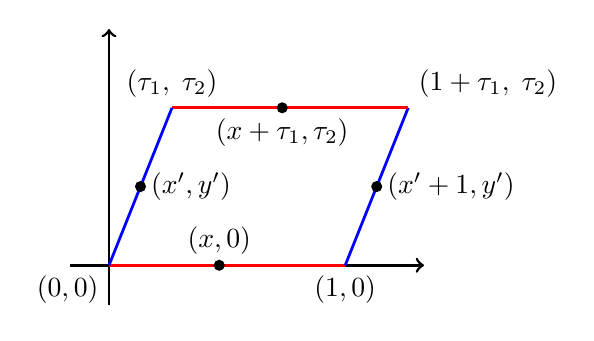
\begin{tikzpicture}[line width=1pt]
			
			% Parameters
			\def\L{3}          
			\def\tauone{0.8}   
			\def\tautwo{2.0}   
			
			% Axes
			\draw[->] (-0.5,0) -- (4,0);
			\draw[->] (0,-0.5) -- (0,3);
			
			% Parallelogram
			%\draw (0,0) -- (\L,0) -- ({\L+\tauone},{\tautwo}) -- (\tauone,\tautwo) -- cycle;
			% Define colors for horizontal and slanted lines
			\draw[red] (0,0) -- (\L,0);                           % Bottom (Horizontal)
			\draw[blue] (\L,0) -- ({\L+\tauone},{\tautwo});       % Right (Slanted)
			\draw[red] ({\L+\tauone},{\tautwo}) -- (\tauone,\tautwo); % Top (Horizontal)
			\draw[blue] (\tauone,\tautwo) -- (0,0);                % Left (Slanted)
			
			% Points and Labels for the Bottom-Top Identification
			\fill (\L/2-0.1, 0) circle (2pt);
			\node[above] at (\L/2-0.1, 0) {$ (x,0) $};
			
			\fill (\L/2-0.1+\tauone, \tautwo) circle (2pt);
			\node[below] at (\L/2-0.1+\tauone, \tautwo) {$ (x+\tau_{1}, \tau_{2}) $};
			
		% Points and Labels for the Left-Right Identification (z ~ z + L)
		\fill (\tauone/2, \tautwo/2) circle (2pt);
		\node[right] at (\tauone/2, \tautwo/2) {$ (x', y') $};
		
		\fill (\L+\tauone/2, \tautwo/2) circle (2pt);
		\node[right] at (\L+\tauone/2, \tautwo/2) {$ (x'+1, y') $};
			
			% Vertex labels
			\node[below left]  at (0,0) {$ (0,0) $};
			\node[below]       at (\L,0) {$ (1,0) $};
			\node[above]       at (\tauone,\tautwo) {$ (\tau_{1},\; \tau_{2}) $};
			\node[above right] at ({\L+\tauone},{\tautwo}) {$ (1+\tau_1,\; \tau_2) $};
			
		\end{tikzpicture}
	\end{minipage}	
	\hfill
	\begin{minipage}{0.45\textwidth}
	\begin{equation}
		\mathcolor{blue}{z \sim z + 1}, \quad \mathcolor{red}{z \sim z + \tau}.
	\end{equation}
	\end{minipage}
\end{center}

The original equation in the $w$-coordinate is:
\begin{equation}
	\frac{2}{\alpha'} \bar{\partial}_w \partial_w G'(w,w') = -2\pi \delta^{(2)}(w-w') + \frac{1}{2\pi\tau_2}.
\end{equation}
Under the coordinate transformation, we get $\bar{\partial}_w \partial_w = \frac{1}{4\pi^2} \bar{\partial}_z \partial_z$ and $\delta^{(2)}(w-w') = \frac{1}{4\pi^2} \delta^{(2)}(z)$, using which we obtain:
\begin{equation}
	\frac{2}{\alpha'} \bar{\partial}_z \partial_z G'(z) = -2\pi \delta^{(2)}(z) + \frac{\pi}{\tau_2}.
\end{equation}
The Laplacian is given by $\nabla_z^2 = 4 \bar{\partial}_z \partial_z$, through which the equation becomes:
\begin{equation}
	\nabla_z^2 G'(z) = 2\alpha' \left[ -2\pi \delta^{(2)}(z) + \frac{\pi}{\tau_2} \right].\label{green:torus}
\end{equation}
The eigenfunctions of $\nabla_z^2$ on the torus are plane waves $\Psi_{\vec{k}}(z) = \frac{1}{\sqrt{N}} e^{i\vec{k} \cdot \vec{z}}$, where the normalization constant $N$ is determined by the orthonormality condition:
\begin{equation}
	\int_{T^2} |\Psi_{\vec{k}}(z)|^2 d^2z = 1 \implies |N|^2 \int_{0}^{\tau_2} \int_{0}^{1} 2 \, dx \, dy = 1.
\end{equation}
Evaluating the integral gives $2\tau_2 |N|^2 = 1$, hence:
\begin{equation}
	N = \frac{1}{\sqrt{2\tau_2}}.
\end{equation}

The periodicities $z \sim z+1$ and $z \sim z+\tau$ restrict the momenta $\vec{k} = (k_x, k_y)$ to:
\begin{equation}
	k_x = 2\pi n, \quad k_y = \frac{2\pi(m - n\tau_1)}{\tau_2}, \quad n, m \in \mathbb{Z}.
\end{equation}
The eigenvalues of the Laplacian are given by:
\begin{equation}
	-|\vec{k}|^2 = -\left[ (2\pi n)^2 + \frac{4\pi^2(m - n\tau_1)^2}{\tau_2^2} \right] = -\frac{4\pi^2 |m - n\tau|^2}{\tau_2^2}.
\end{equation}
Having determined the eigenvalues, we expand $G'(z)$ and the source terms in the eigenfunction basis. The zero-mode of the source term vanishes:
\begin{equation}
	\int_{T^2} \left[ -2\pi \delta^{(2)}(z) + \frac{\pi}{\tau_2} \right]d^2z = -2\pi + \frac{\pi}{\tau_2}(2\tau_2) = 0.
\end{equation}
Therefore, we expand $G'(z) = \sum_{\vec{k} \neq 0} c_{n,m} e^{i\vec{k} \cdot \vec{z}}$ and $\delta^{(2)}(z)=\frac{1}{V_z}\sum_{\vec{k}=0}^{\infty}e^{i\vec{k}\cdot\vec{z}}$, and substitute into the differential equation \eqref{green:torus}:
\begin{equation}
	\sum_{\vec{k} \neq 0} -|\vec{k}|^2 c_{n,m} e^{i\vec{k} \cdot \vec{z}} = 2\alpha' \left( -\frac{2\pi}{N} \sum_{\vec{k} \neq 0} e^{i\vec{k} \cdot \vec{z}} \right).
\end{equation}
Solving for the coefficients $c_{n,m}$:
\begin{equation}
	c_{n,m} = \frac{4\pi \alpha'}{N |\vec{k}|^2} = \frac{4\pi \alpha'}{(2\tau_2) \left( \frac{4\pi^2 |m - n\tau|^2}{\tau_2^2} \right)} = \frac{\alpha' \tau_2}{2\pi |m - n\tau|^2}.
\end{equation}
Hence, the Green's function in the spectral representation is:
\begin{equation}
	G'(z) = \frac{\alpha' \tau_2}{2\pi} \sum_{(n,m) \neq (0,0)} \frac{1}{|m - n\tau|^2} \exp \left[ 2\pi i \left( nx + \frac{m - n\tau_1}{\tau_2}y \right) \right].
\end{equation}
The lattice sum can be evaluated using standard identities, yielding
\begin{equation}
\sum_{(n,m) \neq (0,0)} \frac{1}{|m - n\tau|^2} \exp \left[ 2\pi i \left( nx + \frac{m - n\tau_1}{\tau_2}y \right) \right] = -\frac{\pi}{\tau_2} \ln \left| \frac{\vartheta_1(z, \tau)}{\vartheta'_1(0|\tau)} \right|^2 + \frac{2\pi^2 y^2}{\tau_2^2} + k(\tau,\bar\tau).
\end{equation}
Upon substituting $z = \frac{w-w'}{2\pi}$ back into the equation, we obtain
\begin{align}
G'(w,w')&=-\frac{\alpha'}{2}\ln\left|\frac{\vartheta_1\!\left(\frac{w-w'}{2\pi}\Big|\tau\right)}{\vartheta_1'(0|\tau)}\right|^2+ \frac{\alpha'}{4\pi\tau_2}\,[\Im(w-w')]^2+ k(\tau,\bar\tau).
\end{align}
The constant $k(\tau,\bar\tau)$ is fixed by the orthogonality condition to the zero mode,
\begin{equation}
	\int_{T^2} d^2 w\, G'(w,w') = 0.
\end{equation}
QED.
\end{proof}
\end{tcolorbox}
Parallel to the previous result \eqref{6.2.13}, the expectation value of vertex operators is 
\begin{align}
	& \left\langle\prod_{i=1}^{n}: \mathrel{\me^{\mi k_{i} \cdot X(z_{i}, \bar{z}_{i})}}:\right\rangle \bigg._{\!\!T^{2}} 
	=\mi C_{T^{2}}^{X}(\tau)(2 \pi)^{d} \delta^{d}({\textstyle \sum_{i} k_{i}}) \nonumber \\
	&\qquad \qquad  \times \prod_{i<j}\left|\frac{2 \pi}{\partial_{\nu} \vartheta_{1}(0 \vert \tau)} 
	\vartheta_{1}\biggl(\frac{w_{i j}}{2 \pi} \Big\vert \tau\biggr) \exp 
	\biggl[-\frac{(\operatorname{Im} w_{i j})^{2}}{4 \pi \tau_{2}}\biggr]\right|^{\alpha^{\prime} k_{i} \cdot k_{j}} \:. \label{7.2.4} 
\end{align}
The factor $2 \pi / \partial_{\nu} \vartheta_{1}$ arises from renormalization of self-contractions. 

\subsection*{Scalar Partition Function} 
The total normalization for the sphere was absorbed into the string coupling constant, but we cannot do the same for the torus because it has a non-trivial $\tau$ dependence. 
In fact, we will see significant physics from amplitudes without vertex operators. 
Consider the path integral without vertex operators $\langle 1\rangle_{T^{2}(\tau)} \equiv Z(\tau) $. 
We can view the torus with modulus $\tau$ as a field theory on a circle evolving for Euclidean time $2 \pi \tau_{2}$, translated in the $\sigma^{1}$ direction by $2 \pi \tau_{1}$, and then identifying the ends. 
In the language of operators, this gives the trace 
\begin{align}
	Z(\tau) &=\operatorname{Tr}\Bigl[\exp (2 \pi \mi \tau_{1} P-2 \pi \tau_{2} H)\Bigr] \nonumber \\
	&=(q \bar{q})^{-d / 24} \operatorname{Tr}\Bigl(q^{L_{0}} \bar{q}^{\tilde{L}_{0}}\Bigr) \:. \label{7.2.5} 
\end{align}
Here $q=\exp (2 \pi \mi \tau)$. The momentum $P=L_{0}-\tilde{L}_{0}$ generates translations in $\sigma^{1}$, while the Hamiltonian $H=L_{0}+\tilde{L}_{0}-\frac{1}{24}(c+\tilde{c})$ generates translations in $\sigma^{2}$. 
As in statistical mechanics, this trace weighted by the exponential of the Hamiltonian and other conserved quantities is called the partition function. 

This trace can be split into a sum over occupation numbers $N_{\mu n}$ and $\tilde{N}_{\mu n}$ and an integral over momentum $k^{\mu}$. 
$Z(\tau)$ becomes 
\begin{equation}
	V_{d}(q \bar{q})^{-d / 24} \int \frac{\dif^{d} k}{(2 \pi)^{d}} \exp(-\pi \tau_{2} \alpha^{\prime} k^{2}) 
	\prod_{\mu, n} \sum_{N_{\mu n}, \tilde{N}_{\mu n}=0}^{\infty} q^{n N_{\mu n}} \bar{q}^{n \tilde{N}_{\mu n}} \:. \label{7.2.6} 
\end{equation}
The spacetime volume factor $V_{d}$ comes from the continuous normalization of momentum, where $\sum_{k}$ becomes $V_{d}(2 \pi)^{-d} \int \dif^{d} k$. 
The sum is a geometric series 
\begin{equation}
	\sum_{N=0}^{\infty} q^{n N}=(1-q^{n})^{-1} \:, \label{7.2.7} 
\end{equation}
yielding 
\begin{equation}
	Z(\tau)=\mi V_{d} Z_{X}(\tau)^{d} \:, \label{7.2.8} 
\end{equation}
where 
\begin{equation}
	Z_{X}(\tau)= (4 \pi^{2} \alpha^{\prime} \tau_{2})^{-1 / 2}|\eta(\tau)|^{-2} \:. \label{7.2.9} 
\end{equation}
Here 
\begin{equation}
	\eta(\tau)=q^{1 / 24} \prod_{n=1}^{\infty}(1-q^{n}) \label{7.2.10} 
\end{equation}
is the Dedekind eta function. The factor of $\mi$ comes from the rotation $k^{0} \rightarrow \mi k^{d}$. Also, previously $C_{T^{2}}^{X}(\tau)=Z_{X}(\tau)^{d}$. 

\eqref{7.2.8} is clearly invariant under $\tau \rightarrow \tau+1$. 
The invariance of $Z_{X}$ under $\tau \rightarrow-1 / \tau$ is given by \eqref{7.2.44}, $\eta(-1 / \tau)=(-\mi \tau)^{1 / 2} \eta(\tau)$. 
This generates the entire modular group. Similarly, expectation values with vertex operators are modular covariant. 

This calculation can be performed using holomorphy. The main idea is to obtain a differential equation for $\tau$. 
Consider a torus with modulus $\tau$ and make a small change to the metric $\delta g_{w w}=\epsilon^{*}$. 
The new metric is 
\begin{align}
	\dif s^{2} &= \dif w \dif \bar{w}+\epsilon^{*} \dif w^{2}+\epsilon \dif \bar{w}^{2}  \nonumber \\
	&=(1+\epsilon^{*}+\epsilon) \dif[w+\epsilon(\bar{w}-w)]\, \dif[\bar{w}+\epsilon^{*}(w-\bar{w})]+O(\epsilon^{2}) \:. \label{7.2.11} 
\end{align}
That is, this metric is Weyl equivalent to $\dif w^{\prime} \dif \bar{w}^{\prime}$, where $w^{\prime}=w+\epsilon(\bar{w}-w)$. It has periodicity 
\begin{equation}
	w^{\prime} \cong w^{\prime}+2 \pi \cong w^{\prime}+2 \pi(\tau-2 \mi \tau_{2} \epsilon) \:. \label{7.2.12} 
\end{equation}
The change in the metric is thus equivalent to a change in the modulus 
\begin{equation}
	\delta \tau=-2 \mi \tau_{2} \epsilon \:. \label{7.2.13} 
\end{equation}

After changing the metric, the change in the path integral is 
\begin{align}
	\delta Z(\tau) &= -\frac{1}{2 \pi} \int \dif^{2} w \: \Bigl[\delta g_{\bar{w} \bar{w}} 
	\bigl\langle T_{w w}(w)\bigr\rangle+\delta g_{w w}\bigl\langle T_{\bar{w} \bar{w}}(\bar{w})\bigr\rangle\Bigr] \nonumber \\
	&=-2 \pi \mi\Bigl[\delta \tau \bigl\langle T_{w w}(0)\bigr\rangle - \delta \bar{\tau}\bigl\langle T_{\bar{w} \bar{w}}(0)\bigr\rangle\Bigr] \:. \label{7.2.14} 
\end{align}
In the second line, we used translation invariance to perform the integration. To find the expectation value of the energy-momentum tensor, we use the OPE 
\begin{equation}
	\partial_{w} X^{\mu}(w) \partial_{w} X_{\mu}(0)=-\frac{\alpha^{\prime} d}{2 w^{2}}-\alpha^{\prime} T_{w w}(0)+O(w^{2}) \:. \label{7.2.15} 
\end{equation}
Now, 
\begin{align}
	Z(\tau)^{-1}\langle\partial_{w} X^{\mu}(w) \partial_{w} X_{\mu}(0)\rangle 
	&= \partial_{w} \partial_{w^{\prime}} G^{\prime}(w, \bar{w} ; w^{\prime}, \bar{w}^{\prime})|_{w^{\prime}=0} \nonumber \\
	&=\frac{\alpha^{\prime} d}{2} \frac{\vartheta_{1} \partial_{w}^{2} \vartheta_{1}-\partial_{w} \vartheta_{1} \partial_{w} \vartheta_{1}}{\vartheta_{1}^{2}}+\frac{\alpha^{\prime} d}{8 \pi \tau_{2}} \:, \label{7.2.16} 
\end{align}
where all variables of the theta functions are $(w / 2 \pi, \tau)$. 
It indeed has a double pole at $w=0 $. Carefully expanding the numerator and denominator to order $w^{2}$, the $w^{0}$ term in \eqref{7.2.16} is 
\begin{equation}
	\frac{\alpha^{\prime} d}{6} \frac{\partial_{w}^{3} \vartheta_{1}}{\partial_{w} \vartheta_{1}}+\frac{\alpha^{\prime} d}{8 \pi \tau_{2}} \:. \label{7.2.17} 
\end{equation}
Then the OPE \eqref{7.2.15} gives 
\begin{equation}
	\langle T_{w w}(0)\rangle=\left(-\frac{d}{6} \frac{\partial_{w}^{3} \vartheta_{1}(0 \vert \tau)}{\partial_{w} \vartheta_{1}(0 \vert\tau)}-\frac{d}{8 \pi \tau_{2}}\right) Z(\tau) \:, \label{7.2.18} 
\end{equation}
and the variation \eqref{7.2.14} gives the differential equation 
\begin{equation}
	\partial_{\tau} \ln Z(\tau)=\frac{\pi \mi d}{3} \frac{\partial_{w}^{3} \vartheta_{1}(0 \vert \tau)}{\partial_{w} \vartheta_{1}(0 \vert \tau)}+\frac{\mi d}{4 \tau_{2}} \:. \label{7.2.19} 
\end{equation}
To go further, using 
\begin{equation}
	\partial_{w}^{2} \vartheta_{1}\biggl(\frac{w}{2 \pi} \Big\vert \tau\biggr) = 
	\frac{\mi}{\pi} \partial_{\tau} \vartheta_{1}\biggl(\frac{w}{2 \pi} \Big\vert \tau \biggr) \:. \label{7.2.20} 
\end{equation}
Rewrite \eqref{7.2.19} as 
\begin{equation}
	\partial_{\tau} \ln Z(\tau)=-\frac{d}{3} \partial_{\tau} \ln \partial_{w} \vartheta_{1}(0 \vert \tau)+\frac{\mi d}{4 \tau_{2}} \:. \label{7.2.21} 
\end{equation}
Together with the conjugate equation, this determines $Z(\tau)$ up to a numerical coefficient as 
\begin{equation}
	Z(\tau)=|\partial_{w} \vartheta_{1}(0 \vert \tau)|^{-2 d / 3} \tau_{2}^{-d / 2} \:, \label{7.2.22} 
\end{equation}
The numerical coefficient is determined by other methods. Using \eqref{7.2.43}, we can see it matches \eqref{7.2.8}. 

\subsection*{$bc$ CFT} 

For the ghost CFT, the partition function is also determined by the trace of states. 
On both the left and right sides, there are two sets of creation operators $b_{-n}$ and $c_{-n}$, but they are anticommutative. Thus, occupation numbers can only be 0 or 1. 
Therefore, an oscillator of mode $n$ contributes $(1+q^{n})$. Additionally, there are four ground states, which give 
\begin{align}
	\operatorname{Tr}\Bigl[\exp (2 \pi \mi \tau_{1} P-2 \pi \tau_{2} H)\Bigr] &= 
	(q \bar{q})^{13 / 12} \operatorname{Tr}\Bigl(q^{L_{0}} \bar{q}^{\tilde{L}_{0}}\Bigr) \nonumber \\
	&=4(q \bar{q})^{1 / 12} \prod_{n=1}^{\infty}|1+q^{n}|^{4} \:. \label{7.2.23} 
\end{align}

However, for anticommutative fields, this trace corresponds to a path integral with anti-periodic boundaries in the time direction. To calculate the Faddeev-Popov determinant, the ghost fields must have the same periodicity as the original coordinate transformation, which is periodic. 
Therefore, we need 
\begin{align}
	Z(\tau) &=\operatorname{Tr}\Bigl[(-1)^{F} \exp (2 \pi \mi \tau_{1} P-2 \pi \tau_{2} H)\Bigr] \nonumber \\
	&=0 \:, \label{7.2.24} 
\end{align}
where $(-1)^{F}$ anticommutes with all ghost fields. 
The trace is zero because the ghost numbers of $\lvert \downarrow \downarrow\rangle$ and $\lvert\uparrow \uparrow\rangle$ are opposite to those of $\lvert \uparrow \downarrow\rangle$ and $\lvert\downarrow \uparrow\rangle$ modulo 2. 
From the path integral viewpoint, $Z(\tau)$ is zero due to ghost zero modes arising from the moduli and CKVs. 
They must be saturated by suitable insertions. The simplest non-zero amplitude is 
\begin{equation}
	\Bigl\langle c(w_{1}) b(w_{2}) \tilde{c}(\bar{w}_{3}) \tilde{b}(\bar{w}_{4})\Bigr\rangle \:. \label{7.2.25} 
\end{equation}
In the operator calculation, we write each field in its mode expansion. Only the $n=0$ terms contribute. 
Then \eqref{7.2.25} becomes 
\begin{equation}
	\operatorname{Tr}\Bigl[(-1)^{F} c_{0} b_{0} \tilde{c}_{0} \tilde{b}_{0} \exp (2 \pi \mi \tau_{1} P-2 \pi \tau_{2} H)\Bigr] \:. \label{7.2.26} 
\end{equation}
The operator $c_{0} b_{0} \tilde{c}_{0} \tilde{b}_{0}$ projects onto the ground state $\lvert\uparrow \uparrow\rangle$, so the result is 
\begin{equation}
	(q \bar{q})^{1 / 12} \prod_{n=1}^{\infty}|1-q^{n}|^{4}=|\eta(\tau)|^{4} \:. \label{7.2.27} 
\end{equation}
Note the sign change in the infinite product comes from $(-1)^{F}$ in the trace. Since the CKVs and quadratic differentials on the torus are constant, \eqref{7.2.27} is independent of the position of the ghost fields. 

\subsection*{General CFT} 
For a general CFT % 
\begin{equation}
	Z(\tau)=\sum_{i} q^{h_{i}-c / 24} \bar{q}^{\tilde{h}_{i}-\tilde{c} / 24}(-1)^{F_{i}} \:, \label{7.2.28} % 
\end{equation}
where $i$ runs over all states of the CFT, and $F_{i}$ is the worldsheet fermion number. Invariance under $\tau \rightarrow \tau+1$ requires $h_{i}-\tilde{h}_{i}-\frac{1}{24}(c-\tilde{c})$ to be an integer. % 
Considering the identity operator, this requires $c-\tilde{c}$ to be a multiple of 24. For general operators, this then requires integer spin % 
\begin{equation}
	h_{i}-\tilde{h}_{i} \in \mathds{Z} \:. \label{7.2.29} % 
\end{equation}
Incidentally, CFTs where $c-\tilde{c}$ is not a multiple of 24 must also be interesting. They cannot be modular invariant alone, but with suitable projections, they can be integrated into a modular invariant theory. % 

Invariance under $\tau \rightarrow-1 / \tau$ imposes further restrictions on the spectrum. 
Consider the partition function with $\tau=\mi \ell$, and let $\ell \rightarrow 0 $; the convergence factor $q=\exp (-2 \pi \ell)$ approaches 1. 
Thus, the partition function is determined by the density of the highest weight states. 
Using modular invariance, this equals the partition function with $\tau=\mi / \ell $, where the latter's $q=\exp (-2 \pi / \ell)$ approaches 0. 
Thus, the lowest weight state dominates the sum, which is the identity state with $L_{0}=\tilde{L}_{0}=0$, yielding 
\begin{equation}
	Z(\mi \ell) \stackrel{l \rightarrow 0}{\approx} \exp \left[\frac{\pi(c+\tilde{c})}{12 \ell}\right] \:. \label{7.2.30} 
\end{equation}
The density of highest weight states is thus determined by the central charge. This produces the result for free bosons, where $c=\tilde{c}=d$ counts the number of free bosons. 

\subsection*{Theta Functions} 
The fundamental theta function is 
\begin{equation}
	\vartheta(\nu, \tau)=\sum_{n=-\infty}^{\infty} \exp (\pi \mi n^{2} \tau+2 \pi \mi n \nu) \:. \label{7.2.31} 
\end{equation}
It has periodicities 
\begin{subequations}  \label{7.2.32}
	\begin{align}
		\vartheta(\nu+1, \tau) &= \vartheta(\nu, \tau) \:, \label{7.2.32a}  \\
		\vartheta(\nu+\tau, \tau) &= \exp (-\pi \mi \tau-2 \pi \mi \nu) \vartheta(\nu, \tau) \:, \label{7.2.32b} 
	\end{align}
\end{subequations}
and under modular transformations 
\begin{subequations} \label{7.2.33}
	\begin{align}
		\vartheta(\nu, \tau+1) &= \vartheta(\nu + 1/2, \tau) \:, \label{7.2.33a} \\
		\vartheta(\nu/\tau, -1/\tau) &=(-\mi \tau)^{1 / 2} \exp (\pi \mi \nu^{2} / \tau) \vartheta(\nu, \tau) \:. \label{7.2.33b} 
	\end{align}
\end{subequations}
Aside from the periodicity \eqref{7.2.32}, the theta function has only one zero at $v=\frac{1}{2}(1+\tau)$. It can also be written as an infinite product 
\begin{equation}
	\vartheta(\nu, \tau)=\prod_{m=1}^{\infty}(1-q^{m})(1+z q^{m-1 / 2})(1+z^{-1} q^{m-1 / 2}) \:, \label{7.2.34} 
\end{equation}
where 
\begin{equation}
	q=\exp (2 \pi \mi \tau), \quad z=\exp (2 \pi \mi\nu) \:. \label{7.2.35} 
\end{equation}

We often need the asymptotic behavior of theta functions as $q \rightarrow 0$ or $q \rightarrow 1$. $q \rightarrow 0$ can be read immediately from the product or sum. The behavior at $q \rightarrow 1$ is less obvious but can be obtained from the modular transformation $\tau \rightarrow-1 / \tau$, which relates the two limits via $q \rightarrow \exp \left(4 \pi^{2} / \ln q\right)$. 
It is often useful to define theta functions with characteristics 
\begin{align}
	\vartheta\bigl[\!\begin{smallmatrix} a\\b\end{smallmatrix}\!\bigr]
	(\nu, \tau) &=\exp \Bigl[\pi \mi a^{2} \tau+2 \pi \mi a(\nu+b)\Bigr] \vartheta(\nu+a \tau+b, \tau)  \nonumber \\
	&=\sum_{n=-\infty}^{\infty} \exp \Bigl[\pi \mi(n+a)^{2} \tau+2 \pi \mi(n+a)(\nu+b)\Bigr] \:. \label{7.2.36} 
\end{align}
Other common notations are 
\begin{subequations} \label{7.2.37}
	\begin{align}
		\vartheta_{00}(\nu, \tau)&=\vartheta_{3}(\nu \vert \tau)= 
		\vartheta\bigl[\!\begin{smallmatrix} 0\\0\end{smallmatrix}\!\bigr](\nu, \tau) = \sum_{n=-\infty}^{\infty} q^{n^{2} / 2} z^{n} \:, 
		\label{7.2.37a}  \\
		\vartheta_{01}(\nu, \tau) &= \vartheta_{4}(\nu \vert \tau)=
		\vartheta\bigl[\!\begin{smallmatrix} 0\\1/2\end{smallmatrix}\!\bigr](\nu, \tau)=
		\sum_{n=-\infty}^{\infty}(-1)^{n} q^{n^{2} / 2} z^{n} \:, \label{7.2.37b}\\
		\vartheta_{10}(\nu, \tau) &= \vartheta_{2}(\nu \vert \tau) = 
		\vartheta\bigl[\!\begin{smallmatrix} 1/2\\0\end{smallmatrix}\!\bigr](\nu, \tau)
		=\sum_{n=-\infty}^{\infty} q^{(n-1 / 2)^{2} / 2} z^{n-1 / 2}  \:, \label{7.2.37c} \\
		\vartheta_{11}(\nu, \tau)&=-\vartheta_{1}(\nu \vert \tau) = 
		\vartheta\bigl[\!\begin{smallmatrix} 1/2\\1/2\end{smallmatrix}\!\bigr](\nu, \tau)
		=-\mi \sum_{n=-\infty}^{\infty}(-1)^{n} q^{(n-1 / 2)^{2} / 2} z^{n-1 / 2} \:. \label{7.2.37d} 
	\end{align}
\end{subequations}
Product representations: 
\begin{subequations} \label{7.2.38}
	\begin{align}
		\vartheta_{00}(\nu, \tau) &= \prod_{m=1}^{\infty}(1-q^{m})(1+z q^{m-1/2})(1+z^{-1} q^{m-1/2}) \:, \label{7.2.38a} \\ 
		\vartheta_{01}(\nu, \tau) &= \prod_{m=1}^{\infty}(1-q^{m})(1-z q^{m-1/2})(1-z^{-1} q^{m-1/2}) \:, \label{7.2.38b} \\
		\vartheta_{10}(\nu, \tau) &= 2 \exp (\pi \mi \tau / 4) \cos \pi \nu 
		\prod_{m=1}^{\infty}(1-q^{m})(1+z q^{m})(1+z^{-1} q^{m}) \:, \label{7.2.38c} \\
		\vartheta_{11}(\nu, \tau) &= -2 \exp (\pi \mi \tau / 4) \sin \pi \nu 
		\prod_{m=1}^{\infty}(1-q^{m})(1-z q^{m})(1-z^{-1} q^{m})  \:. \label{7.2.38d} 
	\end{align}	
\end{subequations}
Modular transformations 
\begin{subequations} \label{7.2.39}
	\begin{align}
		\vartheta_{00}(\nu, \tau+1) &= \vartheta_{01}(\nu, \tau)  \:, \label{7.2.39a} \\
		\vartheta_{01}(\nu, \tau+1) &= \vartheta_{00}(\nu, \tau)  \:, \label{7.2.39b} \\
		\vartheta_{10}(\nu, \tau+1) &= \exp (\pi \mi / 4) \vartheta_{10}(\nu, \tau) \:, \label{7.2.39c} \\
		\vartheta_{11}(\nu, \tau+1) &= \exp (\pi \mi / 4) \vartheta_{11}(\nu, \tau) \:, \label{7.2.39d}
	\end{align}
\end{subequations}
and 
\begin{subequations} \label{7.2.40}
	\begin{align}
		\vartheta_{00}(\nu/\tau,-1 / \tau) &= (-\mi \tau)^{1/2} \exp(\pi \mi \nu^{2}/\tau) \vartheta_{00}(\nu, \tau) \:, \label{7.2.40a} \\
		\vartheta_{01}(\nu/\tau,-1 / \tau) &= (-\mi \tau)^{1/2} \exp(\pi \mi \nu^{2}/\tau) \vartheta_{10}(\nu, \tau) \:, \label{7.2.40b} \\
		\vartheta_{10}(\nu/\tau,-1 / \tau) &= (-\mi \tau)^{1/2} \exp(\pi \mi \nu^{2}/\tau) \vartheta_{01}(\nu, \tau) \:, \label{7.2.40c} \\
		\vartheta_{11}(\nu/\tau,-1 / \tau) &=-\mi(-\mi \tau)^{1/2} \exp(\pi \mi \nu^{2}/\tau) \vartheta_{11}(\nu, \tau) \:. \label{7.2.40d} 
	\end{align}
\end{subequations}
We will encounter these functions more frequently in superstrings. 

Theta functions satisfy Jacobi's ``abstruse identity'', which is a special case of the Riemann quartic identity 
\begin{equation}
	\vartheta_{00}^{4}(0, \tau)-\vartheta_{01}^{4}(0, \tau)-\vartheta_{10}^{4}(0, \tau)=0 \:. \label{7.2.41}
\end{equation}
Also note 
\begin{equation}
	\vartheta_{11}(0, \tau)=0 \:. \label{7.2.42} 
\end{equation}
Finally, the Dedekind eta function is 
\begin{equation}
	\eta(\tau)=q^{1 / 24} \prod_{m=1}^{\infty}(1-q^{m})=\left[\frac{\partial_{\nu} \vartheta_{11}(0, \tau)}{-2 \pi}\right]^{1/3} \:. \label{7.2.43} 
\end{equation}
Modular transformations 
\begin{subequations} \label{7.2.44}
	\begin{align}
		\eta(\tau+1) &=\exp (\mi \pi / 12) \eta(\tau)  \:, \label{7.2.44a} \\
		\eta(-1 / \tau) &=(-\mi \tau)^{1 / 2} \eta(\tau) \:. \label{7.2.44b} 
	\end{align}
\end{subequations}

\section{\texorpdfstring{Torus Amplitudes}{7.3 Torus Amplitudes}} \label{sec:7.3} 
We now apply the general result \eqref{5.3.9} to the torus: expressing string scattering amplitudes as integrals with ghost and vertex operator insertions. Two CKVs require one vertex operator to be fixed, so 
\begin{align}
	&S_{T^{2}}(1 ; 2 ; \ldots ; n)  \nonumber \\
	&\quad=\frac{1}{2} \int_{F_{0}} \dif \tau \dif \bar{\tau} \:
	\biggl\langle B \tilde{B} \tilde{c} c \mathscr{V}_{1}(w_{1}, \bar{w}_{1}) 
	\prod_{i=2}^{n} \int \dif w_{i} \dif \bar{w}_{i} \: \mathscr{V}_{i}(w_{i}, \bar{w}_{i})\biggr\rangle_{T^{2}} \:. \label{7.3.1} 
\end{align}
The fundamental region $F_{0}$ is the same as discussed in section \ref{sec:5.1}, and the $\frac{1}{2}$ comes from $w \rightarrow-w$. As with complex field variables, $\dif \tau \dif \bar{\tau}=2 \dif \tau_{1} \dif \tau_{2}$, where $\tau=\tau_{1}+\mi \tau_{2}$. 
The ghost insertion for $\dif \tau$ is 
\begin{align}
	B=\frac{1}{4 \pi}(b, \partial_{\tau}) &=\frac{1}{2 \pi} \int \dif^{2} w \: b_{w w}(w) \partial_{\tau} g_{\bar{w} \bar{w}} \nonumber \\
	&=\frac{\mi}{4 \pi \tau_{2}} \int \dif^{2} w \: b_{w w}(w) \nonumber \\
	& \rightarrow 2 \pi \mi b_{w w}(0) \:. \label{7.3.2} 
\end{align}
We used \eqref{7.2.13}. In the last line, we used the fact that the ghost path integral \eqref{7.2.27} is position-independent. 

The CKG is composed of translations of the torus. Since this group has a finite volume, we do not need to fix it; we can rewrite the amplitude to integrate over all vertex operators and then divide by the volume of the CKG. CKVs are constant, so the expectation value in \eqref{7.3.1} is independent of the position of $c$: we can move $c$ away from $w_{1}$ and place them at some fixed location. For vertex operators, translation invariance implies the amplitude is invariant under $w_{i} \rightarrow w_{i}+w$. 
Average over this translation: 
\begin{equation}
	\int \frac{\dif w \dif \bar{w}}{2(2 \pi)^{2} \tau_{2}} \:, \label{7.3.3} 
\end{equation}
where the denominator is the area of the torus, which is the volume of the CKG. 
Using \eqref{7.3.2} and \eqref{7.3.3}, the amplitude becomes 
\begin{align}
	&S_{T^{2}}(1 ; 2 ; \ldots ; n) \nonumber \\
	&\quad=\int_{F_{0}} \frac{\dif \tau \dif \bar{\tau}}{4 \tau_{2}} 
	\biggl\langle b(0) \tilde{b}(0) \tilde{c}(0) c(0) \prod_{i=1}^{n} \int \dif w_{i} \dif \bar{w}_{i}\: 
	\mathscr{V}_{i}(w_{i}, \bar{w}_{i})\biggr\rangle_{T^{2}} \:. \label{7.3.4} 
\end{align}
Now all vertex operators have equal status. 
\begin{tcolorbox}
	\begin{remark}
		The factor $(4\tau_{2})^{-1}$ in \eqref{7.3.4} comes from $1/2$ in \eqref{7.3.1}, $(2\pi)^{-2}$ in \eqref{7.3.2}, and $(2(2\pi )^2 \tau _2 )^{-1}$ in \eqref{7.3.3}.
	\end{remark}
\end{tcolorbox}

Without the intermediate step of fixing vertex operators, \eqref{7.3.4} can also be derived directly; even without vertex operators, it holds: 
\begin{equation}
	Z_{T^{2}}=\int_{F_{0}} \frac{\dif \tau \dif \bar{\tau}}{4 \tau_{2}} \:
	\Bigl\langle b(0) \tilde{b}(0) \tilde{c}(0) c(0)\Bigr\rangle_{T^{2}} \:. \label{7.3.5} 
\end{equation}
This vacuum amplitude is quite interesting and will be our main goal of study. It not only reveals that the UV behavior of string theory differs from field theory, but also has significant physical meaning itself. 

For 26 flat spacetime dimensions, the path integrals of matter and ghost fields in \eqref{7.3.5} were calculated in the previous section, yielding 
\begin{equation}
	Z_{T^{2}}=\mi V_{26} \int_{F_{0}} \frac{\dif \tau \dif \bar{\tau}}{4 \tau_{2}} \: 
	(4 \pi^{2} \alpha^{\prime} \tau_{2})^{-13}|\eta(\tau)|^{-48} \:. \label{7.3.6} 
\end{equation}
This amplitude has an important property: modular invariance. According to \eqref{7.2.44}, $\tau_{2}|\eta(\tau)|^{4}$ is modular invariant, and it is easy to verify that 
\begin{equation}
	\frac{\dif \tau \dif \bar{\tau}}{\tau_{2}^{2}} \label{7.3.7} 
\end{equation}
is also modular invariant. Note that the exponent $-48$ comes from 24 sets of left-moving and 24 sets of right-moving oscillators. Ghost contributions cancel two sets of oscillators, leaving only the transverse mode contributions. By introducing vertex operators into the expectation value \eqref{7.2.4} and integrating over position, we get the $n$-tachyon amplitude. 
\begin{tcolorbox}
	\begin{itemize}
		\item 
		According to \eqref{7.2.9}, $[Z_{X}(\tau)]^{26}=(4 \pi^{2} \alpha^{\prime} \tau_{2})^{-13}|\eta(\tau)|^{-52}$, and according to \eqref{7.2.27}, $\langle c b \tilde{c} \tilde{b}\rangle=|\eta(\tau)|^{4}$. Multiplying them gives \eqref{7.3.6}. 
		\item Regarding modular invariance, the invariance under $\tau\to\tau+1$ is trivial. Under $\tau\to -1/\tau$, we have $\tau_{2}\to \tau_{2}/|\tau|^{2}$ and $\dif \tau \to (-\tau^{-2})\dif\tau$, which gives the modular invariance of \eqref{7.3.7}. 
	\end{itemize}
\end{tcolorbox}

For a general CFT, the path integral on the torus is expressed by the trace in \eqref{7.2.28}. 
As long as there are $d \geq 2$ non-compact flat dimensions, the ghost fields still cancel two sets of bosonic operators, and the vacuum amplitude is 
\begin{subequations} \label{7.3.8}
	\begin{align}
		Z_{T^{2}} &=V_{d} \int_{F_{0}} \frac{\dif \tau \dif \bar{\tau}}{4 \tau_{2}} \int \frac{\dif^{d} k}{(2 \pi)^{d}}\: 
		\exp (-\pi \tau_{2} \alpha^{\prime} k^{2}) \sum_{i \in \mathscr{H}^{\perp}} q^{h_{i}-1} \bar{q}^{\tilde{h}_{i}-1} \label{7.3.8a}  \\
		&= \mi V_{d} \int_{F_{0}} \frac{\dif \tau \dif \bar{\tau}}{4 \tau_{2}} \: (4 \pi^{2} \alpha^{\prime} \tau_{2})^{-d / 2} 
		\sum_{i \in \mathscr{H}^{\perp}} q^{h_{i}-1} \bar{q}^{\tilde{h}_{i}-1}  \label{7.3.8b}
	\end{align}		
\end{subequations}
Here $\mathscr{H}^{\perp}$ is the closed string Hilbert space excluding ghosts, $\mu=0,1$ oscillators, and non-compact momentum. 
To understand the physics of these amplitudes, it is useful to compare them with the corresponding quantities in field theory, summing over all paths with circle topology. This is given by 
\begin{align}
	Z_{S_{1}}(m^{2}) &=V_{d} \int \frac{\dif^{d} k}{(2 \pi)^{d}} \int_{0}^{\infty} \frac{\dif l}{2 l}  \: 
	\exp [-(k^{2}+m^{2}) l / 2] \nonumber \\
	&=\mi V_{d} \int_{0}^{\infty} \frac{\dif l}{2 l}(2 \pi l)^{-d / 2} \: \exp (-m^{2} l / 2)   \label{7.3.9} 
\end{align}
This can be derived through gauge-fixed point-particle path integrals. The result is intuitive: $l$ is the modulus of the circle, $\frac{1}{2}(k^{2}+m^{2})$ is the Hamiltonian of the worldline, and $2 l$ removes redundant counting from translations and reversing worldline coordinates. 

We now adopt the point-particle result for particles of mass $m^{2}$ and sum over the string spectrum. As stated in Chapter \ref{cha:4}, the physical spectrum corresponds one-to-one with $\mathscr{H}^{\perp}$, where the relationship between mass and transverse weight is 
\begin{equation}
	m^{2}=\frac{2}{\alpha^{\prime}}(h+\tilde{h}-2) \label{7.3.10} 
\end{equation}
subject to the constraint $h=\tilde{h}$. 
This constraint can be written in integral form 
\begin{equation}
	\delta_{h, \tilde{h}}=\int_{-\pi}^{\pi} \frac{\dif \theta}{2 \pi} \exp \Bigl[\mi(h-\tilde{h}) \theta\Bigr] \:. \label{7.3.11} 
\end{equation}
In the above, we assume $h-\tilde{h}$ is an integer. This is true in 26 flat dimensions; as discussed in the previous section, modular invariance is generally important. 
Then 
\begin{align}
	\sum_{i \in \mathscr{H} \perp} Z_{S_{1}}(m_{i}^{2}) &= \mi V_{d} \int_{0}^{\infty} \frac{\dif l}{2 l} 
	\int_{-\pi}^{\pi} \frac{\dif \theta}{2 \pi} \: (2 \pi l)^{-d / 2} \nonumber \\
	&\qquad \qquad  \times \sum_{i \in \mathscr{H}^{\perp}} \exp \Bigl[-(h_{i}+\tilde{h}_{i}-2) l / \alpha^{\prime}
	+\mi(h_{i}-\tilde{h}_{i}) \theta\Bigr]  \nonumber \\
	&=\mi V_{d} \int_{R} \frac{\dif \tau \dif \bar{\tau}}{4 \tau_{2}}\: (4 \pi^{2} \alpha^{\prime} \tau_{2})^{-d / 2} 
	\sum_{i \in \mathscr{H} \perp} q^{h_{i}-1} \bar{q}^{\tilde{h}_{i}-1} \:, \label{7.3.12} 
\end{align}
where $\theta+\mi l / \alpha^{\prime}=2 \pi \tau$. 
Integration region $R$: 
\begin{equation}
	R: \quad \tau_{2}>0, \quad |\tau_{1}|<\frac{1}{2} \:. \label{7.3.13} 
\end{equation}

We now interpret this result. A single point-particle amplitude \eqref{7.3.9} diverges as $l \rightarrow 0$. This is the standard UV divergence of quantum field theory. Summing over the string spectrum as in \eqref{7.3.12} only worsens the situation, as all string contributions have the same sign. However, comparing \eqref{7.3.12} with the actual string amplitude \eqref{7.3.8}, they are very similar with one significant difference. 
The integration regions differ: in string theory, it is the fundamental domain 
\begin{equation}
	F_{0}: \quad|\tau|>1, \quad |\tau_{1}|<\frac{1}{2}, \quad \tau_{2}>0 \label{7.3.14} 
\end{equation}
The UV divergence region is bypassed. We can also see this from the momentum integral \eqref{7.3.8a}. 

Another possible divergence comes from the limit $\tau_{2} \rightarrow \infty$, when the torus becomes very long. 
In this region, the string amplitude in 26 dimensions has the expansion 
\begin{equation}
	\mi V_{26} \int^{\infty} \frac{\dif \tau_{2}}{2 \tau_{2}} \:(4 \pi^{2} \alpha^{\prime} \tau_{2})^{-13}
	\Bigl[\exp (4 \pi \tau_{2})+24^{2}+\cdots\Bigr] \:, \label{7.3.15} 
\end{equation}
The asymptotic behavior is controlled by the lightest string states. The first term in the series diverges, and from the field theory perspective, the explanation is obvious: the series is arranged in order of increasing mass squared. 
The first term comes from the tachyon, and the divergence arises from the positive exponent in the path sum \eqref{7.3.9}. This is a product of a theory containing tachyons and does not affect more realistic theories. Incidentally, this path sum can be defined by analytic continuation of positive mass squared, but problems remain—the continued energy density is complex. This signifies instability, where the tachyon field rolls down its inverted potential. For general CFT, \eqref{7.3.12} becomes 
\begin{equation}
	\mi V_{d} \int^{\infty} \frac{\dif \tau_{2}}{2 \tau_{2}} \: (4 \pi^{2} \alpha^{\prime} \tau_{2})^{-d / 2} 
	\sum_{i} \exp (-\pi \alpha^{\prime} m_{i}^{2} \tau_{2}) \:. \label{7.3.16} 
\end{equation}
Since tachyons always appear in bosonic string theory, this is divergent; without tachyons, it would be convergent. 

The torus exemplifies a general principle that holds for all string amplitudes: there is no UV region in moduli space giving rise to high-energy divergences. All limits are controlled by the lightest string states, i.e., long-range physics. For the torus with vertex operators, the $\tau$ integral is still truncated as above. But more limits exist when vertex operators approach each other. The same general principle applies to them, which we will discuss further in Chapter \ref{cha:9}. 

By truncating the $l$ integral, we can attempt to remove UV divergences in field theory. 
Similarly, one can try to make similar corrections to string theory. For example, replacing the usual fundamental domain $F_{0}$ with $|\tau_{1}| \leq \frac{1}{2}$, $\tau_{2}>1$. 
However, in either case, this would destroy the consistency of the theory: non-physical negative-norm states will no longer decouple. We saw in the general discussion of section \ref{sec:5.4} that the coupling of BRST-null states is proportional to the total derivative on moduli space. 
For the fundamental domain $F_{0}$, the boundaries I and $\mathrm{I}^{\prime}$, and II and $\mathrm{II}^{\prime}$ are equivalent, so boundary terms cancel. Modifying the integration region would introduce real boundaries, and surface terms on moduli space would no longer cancel. Thus, there would be non-zero amplitudes for null states and an inconsistent quantum theory. If we make a brute-force truncation to make a gravity theory finite, this is a direct analogy of the consequence: it is extremely difficult to do so without destroying local spacetime symmetry and making the theory inconsistent. 
String theory provides a subtle way that softens short-distance behavior and eliminates divergences without losing spacetime gauge invariance. 

\subsection*{Physics of the Vacuum Amplitude} 
Besides exemplifying the behavior of string amplitudes, the one-loop vacuum amplitude has an interesting physical interpretation. In point-particle theory, "vacuum" paths consist of any $n$ non-intersecting circles. Permutation symmetry introduces a factor $1/n!$, and summing over $n$ gives 
\begin{equation}
	\bm{Z}_{\mathrm{vac}}(m^{2})=\exp \Bigl[Z_{S_{1}}(m^{2})\Bigr] \:. \label{7.3.17} 
\end{equation}
Switching to canonical field theory, 
\begin{align}
	Z_{\mathrm{vac}}(m^{2}) &= \langle 0|\exp (-\mi H T)| 0\rangle \nonumber \\
	&=\exp (-\mi \rho_{0} V_{d}) \:, \label{7.3.18} 
\end{align}
where $\rho_{0}$ is the vacuum energy density: 
\begin{equation}
	\rho_{0}=\frac{\mi}{V_{d}} Z_{S_{1}}(m^{2}) \:. \label{7.3.19} 
\end{equation}

The $l$ integral in $Z_{S_{1}}(m^{2})$ diverges as $l \rightarrow 0 $. In renormalizable field theory, this is cancelled by counterterms or supersymmetry. 
We truncate the integral $l \geq \epsilon$ and then take $\epsilon \rightarrow 0$, but discard the divergent terms. Under this treatment, 
\begin{equation}
	\int_{0}^{\infty} \frac{\dif l}{2 l} \exp [-(k^{2}+m^{2}) l / 2] \rightarrow-\frac{1}{2} \ln(k^{2}+m^{2}) \label{7.3.20} 
\end{equation}
\begin{tcolorbox}
	\begin{proof}
		Use the incomplete gamma function integral:
		\begin{equation}
			\lim_{\epsilon\to0}\int_{\epsilon}^{\infty}\frac{dl}{2l}e^{-\frac{xl}{2}}=\lim_{\epsilon\to0}\frac{1}{2}\Gamma\left(0,\frac{\epsilon x}{2}\right)\approx \lim_{\epsilon\to0}\frac{-\gamma -\ln(\epsilon x)+\epsilon x}{2}
		\end{equation}
	\end{proof}
\end{tcolorbox}
and 
\begin{equation}
	\mi \int_{0}^{\infty} \frac{\dif l}{2 l} \int_{-\infty}^{\infty} \frac{\dif k^{0}}{2 \pi} \: 
	\exp [-(k^{2}+m^{2})l/2] \rightarrow \frac{\omega_{\mathbf{k}}}{2} \:, \label{7.3.21} 
\end{equation}
where $\omega_{\mathbf{k}}^{2}=\mathbf{k} \cdot \mathbf{k}+m^{2}$. 
Using \eqref{7.3.21}, the vacuum energy density becomes 
\begin{equation}
	\rho_{0}=\int \frac{\dif^{d-1} \mathbf{k}}{(2 \pi)^{d-1}} \: \frac{\omega_{\mathbf{k}}}{2} \:, \label{7.3.22} 
\end{equation}
which is exactly the sum of the zero-point energies of each mode of the field. We encountered a similar sum in section \ref{sec:1.3}, though that was on the worldsheet. 

Describing quantum field theory as a sum of particle paths may be less familiar than describing it as a sum over field histories, but they are equivalent. 
Specifically, the free path integral of field theory can be found in modern field theory textbooks: 
\begin{align}
	\ln \bm{Z}_{\mathrm{vac}}(m^{2}) &=-\frac{1}{2} \operatorname{Tr} \ln (-\partial^{2}+m^{2}) \nonumber \\
	&=-\frac{V_{d}}{2} \int \frac{\dif^{d} k}{(2 \pi)^{d}} \ln (k^{2}+m^{2}) \:. \label{7.3.23} 
\end{align}
Using \eqref{7.3.20}, this is identical to the path sum result \eqref{7.3.9}. 

In older quantum field theory books, vacuum amplitudes like \eqref{7.3.18} were usually considered irrelevant. 
If the scattering amplitudes are considered in a fixed background and gravity is ignored, this is correct. But vacuum energy density is significant in at least two cases. First, to compare the energy densities of different states to determine which is the vacuum ground state. For example, electroweak $S U(2) \times U(1)$ symmetry breaking is likely determined by quantum corrections to vacuum energy density. This was the original motivation for the Coleman-Weinberg formula \eqref{7.3.23}. Extending to arbitrary spin, 
\begin{equation}
	\rho_{0}=\frac{\mi}{V_{d}} \sum_{i}(-1)^{\mathbf{F}_{i}} Z_{S_{1}}(m_{i}^{2}) \:. \label{7.3.24} 
\end{equation}
The sum is taken over all physical particle states. Each polarization is counted separately, giving a factor $2 s_{i}+1$ for spin $s_{i}$ in 4 dimensions. Here $\mathbf{F}_{i}$ is the spacetime fermion number, so fermions contribute with the opposite sign. 

The second case is consideration of coupling with gravity. Vacuum energy provides the source term in the Einstein equations—the cosmological constant—and thus has observable effects. In fact, this cosmological constant is a major challenge. Because real spacetime is approximately flat and static, its value must be very small: 
\begin{equation}
	|\rho_{0}| \lesssim 10^{-44} \mathrm{GeV}^{4} \:. \label{7.3.25} 
\end{equation}
If only the vacuum energy contribution of known particles is considered (roughly below the electroweak scale), the zero-point energy is already about 
\begin{equation}
	m_{\mathrm{ew}}^{4} \approx 10^{8} \mathrm{GeV}^{4} \:, \label{7.3.26} 
\end{equation}
which is 52 orders of magnitude higher than reality. The potential energy of the Higgs field and QCD vacuum energy are also too large. Finding a mechanism that cancels the net cosmological constant with great precision has proven difficult. For example, in supersymmetric theories, the contributions of degenerate bosons and fermions in the sum \eqref{7.3.24} cancel. But supersymmetry has not yet been seen in nature, so it must be a broken symmetry. Then the cancellation is imperfect, again leaving at least $m_{\mathrm{ew}}^{4} $ as a remainder. The cosmological constant problem is one of the most persistent difficulties. 
Thus, one of the best clues likely lies in finding a unified theory containing gravity. 

What about the cosmological constant problem in string theory? At the string tree level, we have a consistent theory compatible with flat metrics, so the cosmological constant is zero. In fact, when we chose 26 dimensions, we adjusted it manually. From the spacetime action \eqref{3.7.20}, it is evident that otherwise, there would be a tree potential proportional to $D-26$. The one-loop vacuum energy density in bosonic string amplitudes is non-zero and must be on the scale of the string (ignoring tachyon divergence). In 4 dimensions, this corresponds to $10^{72} \mathrm{GeV}^{4}$, which is still too large. 
In supersymmetric string theory, there will be some amount of cancellation, but in a realistic theory with broken supersymmetry, a remainder of at least $m_{\mathrm{ew}}^{4}$ can still be expected. 

The cosmological constant problem tells us that there is still something about the vacuum we do not understand, both in field theory and in string theory. 

\section{\texorpdfstring{Open and Unoriented One-loop Amplitudes}{7.4 Open and Unoriented One-loop Amplitudes}} \label{sec:7.4} % 

\subsection*{Cylinder} % 
The results for the torus can be immediately extended to other surfaces with zero Euler number. % 
For example, the vacuum amplitude from the cylinder in oriented theory is 
\begin{align}
	Z_{C_{2}} &=\int_{0}^{\infty} \frac{\dif t}{2 t} \operatorname{Tr}_{\mathrm{o}}^{\prime}[\exp(-2 \pi t L_{0})]
	=\mi V_{d} \int_{0}^{\infty} \frac{\dif t}{2 t}\: (8 \pi^{2} \alpha^{\prime} t)^{-d / 2} 
	\sum_{i \in \mathscr{H}_{0}^{\perp}} \exp[-2 \pi t(h_{i}-1)] \nonumber \\
	&\rightarrow \mi V_{26} n^{2} \int_{0}^{\infty} \frac{\dif t}{2 t}\,(8 \pi^{2} \alpha^{\prime} t)^{-13} \eta(\mi t)^{-24} \:. \label{7.4.1} 
\end{align}
This can be obtained either by writing the path integral in terms of ghost zero modes, as we did for the torus, or by guessing it, summing the point-particle result over the open string spectrum. In the first line, the trace is over the entire open string CFT, and the prime indicates ghost zero modes are dropped. In the last line, the trace is over 26 flat dimensions and $n$ Chan-Paton degrees of freedom. Introducing tachyon vertex operators is straightforward. 

The $t \rightarrow \infty$ limit of the cylinder is very similar to the $\tau_{2} \rightarrow \infty$ limit of the torus. The cylinder looks like a long strip, and the leading order approximation is given by the lightest open string states. 
As with closed strings, there are divergences, but only from the open string tachyon. 

\begin{figure}[!htbp]
	\begin{center}
		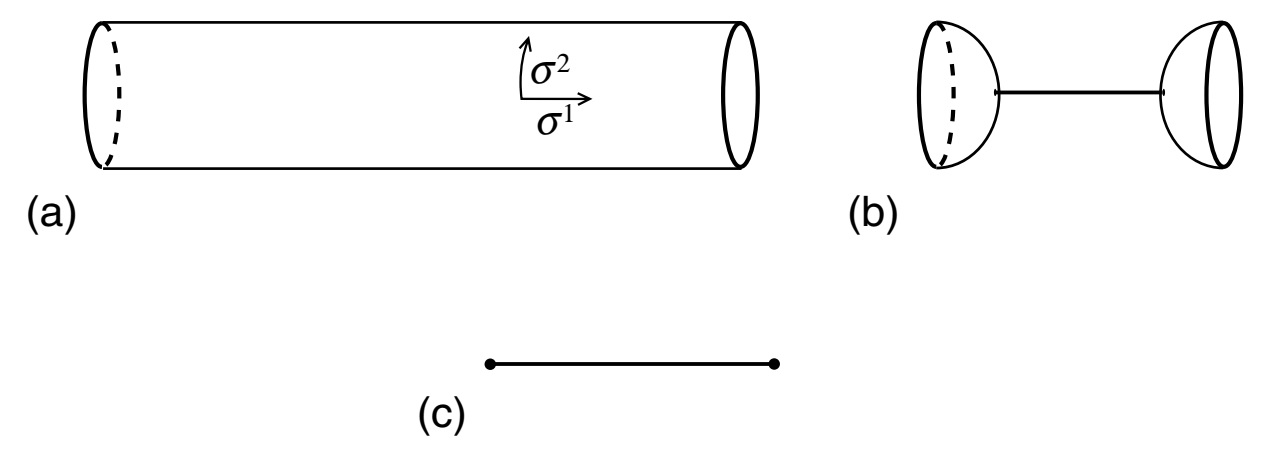
\includegraphics[width=0.8\textwidth]{figure/Fig7.1.jpg}\\
		\caption{(a) Cylinder in the small $t$ limit. (b) Amplitude decomposed into disk tadpole amplitudes and a closed string propagator. (c) Analogous field theory Feynman diagram. Heavy particles are analogous to tadpoles.}\label{Fig7.1} 
	\end{center}
\end{figure}

The $t \rightarrow 0$ limit is quite interesting. Unlike the torus, there is no modular group, and the integration limits cannot be truncated, so UV divergences of field theory still manifest. 
However, we will see that, like all divergences in string theory, this should actually be interpreted as a long-range effect. In the $t \rightarrow 0$ limit, this cylinder is very long, as shown in Figure \ref{Fig7.1}a. It looks like a closed string emerging from vacuum, propagating a certain distance, and then disappearing back into the vacuum. 
To make it more obvious, using the modular transformation \eqref{7.2.44} 
\begin{equation}
	\eta(\mi t)=t^{-1 / 2} \eta(\mi / t) \label{7.4.2} 
\end{equation}
and changing the variable to $s=\pi / t$, the result is 
\begin{equation}
	Z_{C_{2}}=\mi \frac{V_{26} n^{2}}{2 \pi(8 \pi^{2} \alpha^{\prime})^{13}} \int_{0}^{\infty} \dif s\: \eta(\mi s / \pi)^{-24} \:. \label{7.4.3} 
\end{equation}
Rescaling the metric by $1 / t$, the cylinder has a closed string circumference $2 \pi$, and the cylinder length is $s$. Expanding 
\begin{align}
	\eta(\mi s / \pi)^{-24} &=\exp (2 s) \prod_{n=1}^{\infty}[1-\exp (-2 n s)]^{-24} \nonumber \\
	&=\exp (2 s)+24+O(\exp (-2 s)) \:, \label{7.4.4} 
\end{align}
this is exactly the expected asymptotic form for an expansion in the complete closed string basis. 
In other words, if we consider $\sigma^{2}$ as worldsheet time and $\sigma^{1}$ as worldsheet distance, Figure \ref{Fig7.1}a is a very short open string loop. If we swap their roles, it is a very long closed string worldline, with both the beginning and end on the boundary circles. In Euclidean path integrals, both descriptions are usable and useful in different limits of moduli space. 

The leading order contribution to the vacuum amplitude comes from the closed string tachyon. 
This is uninteresting and can be defined through analytic continuation, 
\begin{equation}
	\int_{0}^{\infty} \dif s\:  \exp (\beta s) \equiv-\frac{1}{\beta} \:. \label{7.4.5} 
\end{equation}
The second term comes from massless closed string states, which even with continuation give a divergence of the form $1 / 0$. To see the origin of this divergence, dissociate the process as in Figure \ref{Fig7.1}b. As we saw in section \ref{sec:6.6}, there is a non-zero amplitude for a closed string vertex operator on a disk. 
The tadpole diagram corresponds to a closed string disappearing or appearing in the vacuum. In momentum space, the massless propagator is proportional to $1 / k^{2}$. Here, momentum conservation requires the momentum of the closed string emerging from vacuum to be zero, so the propagator diverges. 

The same type of divergence exists in quantum field theory. Consider a massless scalar field $\phi$ with a linear term for $\phi$ in the Lagrangian. Then there will be a vertex connected to only one propagator, and Figure \ref{Fig7.1}c exists. This divergence is due to the intermediate propagator being 
\begin{equation}
	\frac{1}{k^{2}}\bigg|_{k^{\mu}=0} \:. \label{7.4.6} 
\end{equation}
Since propagator poles correspond to long propagation distances in spacetime, this is a long-range (infrared) divergence. 
UV and IR divergences in quantum field theory have very different origins. UV divergences usually signal theory failure, requiring new physics at some short scale. IR divergences usually mean the question asked is wrong, or the method of expansion is wrong. This is the case here too. In general perturbation theory, we expand around $\phi(x)=0$ or some other field configuration. For the action 
\begin{equation}
	-\frac{1}{g^{2}} \int \dif^{d} x \: \left(\frac{1}{2} \partial_{\mu} \phi \partial^{\mu} \phi+g \Lambda \phi\right) \:, \label{7.4.7} 
\end{equation}
the equation of motion 
\begin{equation}
	\partial^{2} \phi=g \Lambda \label{7.4.8} 
\end{equation}
does not allow $\phi(x)=0$ as a solution. 
We must expand around a solution of \eqref{7.4.8}; any such solution must be position-dependent. The corresponding amplitude has no divergence, even if the right side is a perturbation (we introduced a suitable factor $g$ to the disk), because it is a singular perturbation. Specifically, the correct background breaks some Poincaré symmetries of the zero-order solution. 

The situation in string theory is the same. The disk tadpole is the source 
\begin{equation}
	-\Lambda \int \dif^{26} x\: (-G)^{1 / 2} \me^{-\tilde{\Phi}} \:, \label{7.4.9} 
\end{equation}
which is a source for the dilaton and metric. Expanding around the solution of the corresponding field equations (no longer constant) gives effective amplitudes. 
The details are somewhat complex and will be further discussed in Chapter \ref{cha:9}. Incidentally, in superstring theory, if the tree-level background is invariant under supersymmetry, it usually has no loop corrections. 

The pole \eqref{7.4.6} is the same type of divergence we encountered in tree amplitudes, corresponding to resonances propagating over long spacetime distances. If we add open string vertex operators at each end of the cylinder so that it represents an open string one-loop amplitude, the momentum $k^{\mu}$ flowing from one boundary to another is generally non-zero. 
Then the large $s$ limit \eqref{7.4.4} introduces the factor 
\begin{equation}
	\exp (-\alpha^{\prime} k^{2} s / 2)\:, \label{7.4.10} 
\end{equation}
and the divergence becomes a momentum pole, representing an open string scattering into a closed string intermediate state. Thus, as claimed in Chapter \ref{cha:3}, open string theory must simultaneously incorporate closed strings. The mechanism for removing UV divergences is different in open and closed strings. In closed strings, it is an effective truncation on modular integrals; in open strings, in the form of long spacetime distances, it is reinterpreted as a dangerous limit of moduli space. 

In \eqref{7.4.1}, we associated the path integral on the cylinder with the open string spectrum by cutting the path integral with $\sigma^{2}$ as time. 
It can also be obtained through closed strings, where $\sigma^{1}$ is time. Let $\sigma^{2}$ have period $2 \pi$ , with boundaries at $\sigma^{1}=0, s$. The closed string emerges in some state $|B\rangle$ at $\sigma^{1}=0$, and then disappears in the same way at $\sigma^{1}=s $. 
Introducing a measure insertion, the path integral is proportional to 
\begin{equation}
	\langle B|c_{0} b_{0} \exp [-s(L_{0}+\tilde{L}_{0})]| B\rangle \:. \label{7.4.11} 
\end{equation}
The fact that $\partial_{1} X^{\mu}, c^{1}$ and $b_{12}$ are zero on the boundary determines the state $|B\rangle$. 
In Hamiltonian form, they must annihilate $|B\rangle$; in terms of Laurent coefficients, 
\begin{equation}
	(\alpha_{n}^{\mu}+\tilde{\alpha}_{-n}^{\mu})|B\rangle=(c_{n}+\tilde{c}_{-n})|B\rangle=(b_{n}-\tilde{b}_{-n})|B\rangle=0, \quad \text { all } n\:. \label{7.4.12} 
\end{equation}
This gives 
\begin{equation}
	|B\rangle \propto (c_{0}+\tilde{c}_{0}) \exp \biggl[-\sum_{n=1}^{\infty}(n^{-1} \alpha_{-n} \cdot \tilde{\alpha}_{-n}+b_{-n} \tilde{c}_{-n}+\tilde{b}_{-n} c_{-n})\biggr]|0 ; 0\rangle \:. \label{7.4.13} 
\end{equation}
Using this in \eqref{7.4.11} yields \eqref{7.4.3}, with the normalization of $|B\rangle$ yet to be determined. This representation is very useful for analyzing the $t \rightarrow 0$ limit and closed string poles. 

By comparing string calculations with field theory, we can determine the disk tadpole $\Lambda$, but it will be more convenient to treat it as a special case of a more general result in the next chapter. 

\subsection*{Klein Bottle} 

The vacuum amplitude from the Klein bottle is 
\begin{align}
	Z_{K_{2}} &=\int_{0}^{\infty} \frac{\dif t}{4 t}\: \operatorname{Tr}_{\mathrm{c}}^{\prime} 
	\Bigl\{\Omega \exp [-2 \pi t (L_{0}+\tilde{L}_{0})]\Bigr\}  \nonumber \\
	&=\mi V_{d} \int_{0}^{\infty} \frac{\dif t}{4 t} \:(4 \pi^{2} \alpha^{\prime} t)^{-d / 2} 
	\sum_{i \in \mathscr{H}_{c}^{\perp}} \Omega_{i} \exp [-2 \pi t(h_{i}+\tilde{h}_{i}-2)] \:, \label{7.4.14} 
\end{align}
where the notation of the cylinder \eqref{7.4.1} is adopted. 
Compared with the torus of the oriented theory, this has an extra factor of $\frac{1}{2}$, coming from the projection operator $\frac{1}{2}(1+\Omega)$. For the same reason, the torus and cylinder amplitudes in unoriented theory both have an extra factor of $\frac{1}{2}$. This can also be seen as arising from the extra gauge invariance $w \rightarrow \bar{w}$. To calculate the trace in 26 flat dimensions, note that the only diagonal elements of $\Omega$ are those states where left-movers and right-movers are the same, and these states contribute $\Omega=+1 $. Thus, the trace is actually taken only on one side, which is the same as the open string amplitude, except that the weight is doubled because left and right contributions are identical. 
The result is 
\begin{equation}
	Z_{K_{2}} \rightarrow \mi V_{26} \int_{0}^{\infty} \frac{\dif t}{4 t}\: (4 \pi^{2} \alpha^{\prime} t)^{-13} \eta(2 \mi t)^{-24} \:. \label{7.4.15} 
\end{equation}

\begin{figure}[!htbp]
	\begin{center}
		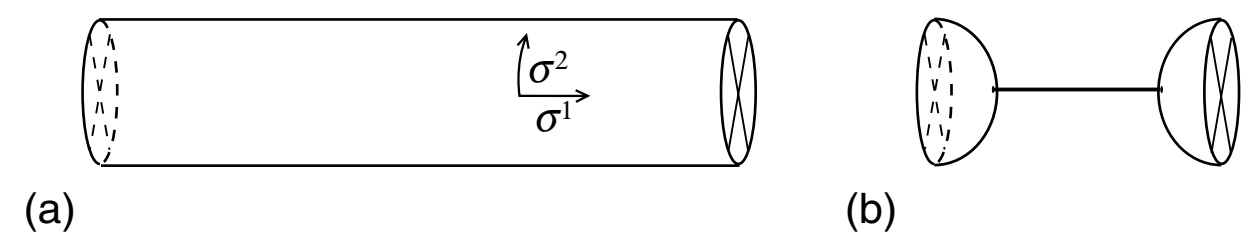
\includegraphics[width=0.8\textwidth]{figure/Fig7.2.jpg}\\
		\caption{(a) In the small $t$ limit, the Klein bottle becomes a cylinder with crosscaps at both ends. (b) Amplitude decomposed into $R P_{2}$ and $D_{2}$ tadpole amplitudes and a closed string propagator.}\label{Fig7.2} 
	\end{center}
\end{figure}

The modulus $t$ has the same range $0<t<\infty$ as for the cylinder, so the $t \rightarrow 0$ divergence is the same. 
Similarly, the $1 / 0$ pole can have a long-range explanation in the form of a closed string pole. To see this, consider the regions 
\begin{subequations} \label{7.4.16}
	\begin{align}
		&0 \leq \sigma^{1} \leq 2 \pi, \qquad 0 \leq \sigma^{2} \leq 2 \pi t  \:, \label{7.4.16a} \\
		&0 \leq \sigma^{1} \leq \pi, \qquad 0 \leq \sigma^{2} \leq 4 \pi t \:. \label{7.4.16b} 
	\end{align}		
\end{subequations}
Both are fundamental regions for the equivalence relation 
\begin{equation}
	w \cong w+2 \pi \cong-\bar{w}+2 \pi \mi t \label{7.4.17} 
\end{equation}
In \eqref{7.4.16a}, the left and right edges are periodically equivalent, while the top and bottom edges are equivalent after parity inversion, which explains the closed string loop with weight $\Omega $. For \eqref{7.4.16b}, the equivalence relation \eqref{7.4.17} simultaneously implies 
\begin{equation}
	w \cong w+4 \pi \mi t, \qquad w+\pi \cong-(\bar{w}+\pi)+2 \pi \mi t \:. \label{7.4.18} 
\end{equation}
It follows that the upper and lower edges of the region \eqref{7.4.16b} are periodically equivalent. After translating half the length of the left edge, the inversion through that edge is equivalent to itself. Similarly for the right edge: this is the definition of a crosscap. Thus we have the interpretation of Figure \ref{Fig7.2}a. Rescaling by $1 / 2 t$, the cylinder base length is $2 \pi$, height $s=\pi / 2 t$, and both ends are connected to crosscaps. 
After modular transformation, the amplitude becomes 
\begin{equation}
	Z_{K_{2}}=\mi \frac{2^{26} V_{26}}{4 \pi(8 \pi^{2} \alpha^{\prime})^{13}} \int_{0}^{\infty} \dif s\: \eta(\mi s / \pi)^{-24} \:. \label{7.4.19} 
\end{equation}
All discussions regarding divergences of the cylinder can be applied to the Klein bottle. The difference is that the tadpole diagrams come from the projective plane rather than the disk. 

\subsection*{M\"{o}bius Strip} 

For the M\"{o}bius strip, 
\begin{equation}
	Z_{M_{2}}=\mi V_{d} \int_{0}^{\infty} \frac{\dif t}{4 t} (8 \pi^{2} \alpha^{\prime} t)^{-d / 2} 
	\sum_{i \in \mathscr{H}_{0}^{\perp}} \Omega_{i} \exp [-2 \pi t(h_{i}-1)] \label{7.4.20} 
\end{equation}
It differs from the cylinder result only by $\Omega$ and the $\frac{1}{2}$ of the projection operator. 
In 26 flat dimensions, the effect of the operator $\Omega$ in the trace is: there is an extra $-1$ on even mass levels, plus a proper count of Chan-Paton factors. Thus, the trace of oscillators is 
\begin{equation}
	\exp (2 \pi t) \prod_{n=1}^{\infty}[1-(-1)^{n} \exp (-2 \pi n t)]^{-24}=\vartheta_{00}(0,2 \mi t)^{-12} \eta(2 \mi t)^{-12} \:. \label{7.4.21} 
\end{equation}
For $S O(n)$ theory, $\frac{1}{2} n(n+1)$ symmetric states have $\Omega=+1$, while $\frac{1}{2} n(n-1)$ antisymmetric states have $\Omega=-1$, giving a net contribution of $n$. For $S p(k)$ theory, it is the opposite, giving $-n$ (in our notation $n=2 k$ Chan-Paton states). 
Then the amplitude is 
\begin{equation}
	Z_{M_{2}}=\pm \mi n V_{26} \int_{0}^{\infty} \frac{\dif t}{4 t} \: (8 \pi^{2} \alpha^{\prime} t)^{-13} 
	\vartheta_{00}(0,2 \mi t)^{-12} \eta(2 \mi t)^{-12} \:. \label{7.4.22} 
\end{equation}


\begin{figure}[!htbp]
	\begin{center}
		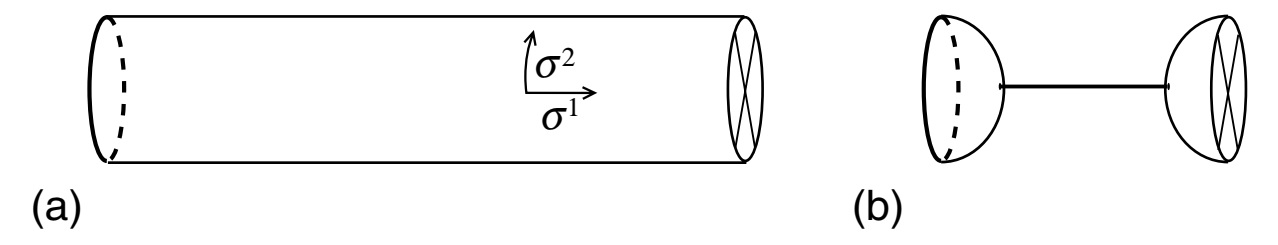
\includegraphics[width=0.8\textwidth]{figure/Fig7.3.jpg}\\
		\caption{(a) In the small $t$ limit, the Möbius strip becomes a cylinder with a crosscap at one end. (b) Amplitude decomposed into $D_{2}$ and $R P_{2}$ tadpole amplitudes and a closed string propagator.}\label{Fig7.3} 
	\end{center}
\end{figure}

By the same construction as for the Klein bottle, the M\"{o}bius strip can also be represented as a cylinder with a base, where only one end is a crosscap, as shown in Figure \ref{Fig7.3}a. The cylinder length is now $s=\pi / 4 t$. 
Through modular transformation, the amplitude is 
\begin{equation}
	Z_{M_{2}}=\pm 2 \mi n \frac{2^{13} V_{26}}{4 \pi(8 \pi^{2} \alpha^{\prime})^{13}}
	\int_{0}^{\infty} \dif s \: \vartheta_{00}(0,2 \mi s / \pi)^{-12} \eta(2 \mi s / \pi)^{-12} \:. \label{7.4.23} 
\end{equation}
As with the cylinder, this can also be written as an operator expression, with one boundary state in \eqref{7.4.11} replaced by a similar crosscap state $|C\rangle $. This is also a $t \rightarrow 0$ divergence; it corresponds to the process in Figure \ref{Fig7.3}a, with one end from the disk and the other from the projective plane. 
In unoriented theory, the divergences of these three surfaces combine into % 
\begin{equation}
	\mi \frac{24 V_{26}}{4 \pi(8 \pi^{2} \alpha^{\prime})^{13}}(2^{13} \mp n)^{2} \int_{0}^{\infty} \dif s\:. \label{7.4.24} % 
\end{equation}
That is, the total tadpole is proportional to $2^{13} \mp n $. % 
For the gauge group $SO(2^{13})=S O(8192)$, this is zero. The tadpole from the disk and the tadpole from the projective plane cancel each other. In bosonic string theory, this might not have special meaning, but in superstrings, there is indeed a similar cancellation for $SO(32)$. %